\chapter{Introduction}
Digits recognition is a well-known and thoroughly explained subject in the image processing field. The outcome of those studies has significant impact for many aspects in people's lives. We used to provide credit curd number by hand some time ago, until the cell phones started to do it for us with the help of the camera. Automatic opening the gate basing on the plates numbers for entitled cars in the parking or motorway gates for those whose owners paid the toll upfront. These examples are just a pick of an iceberg of the potential digits recognition use cases. 

Image recognition and deep learning algorithms became globally available not only for scientists, but also for ordinary individuals, especially because of high level libraries like Tensorflow or PyTorch where the exact knowledge of how the particular algorithm works is often irrelevant for the sake of the API. Developer has to invoke proper function with the desired parameters, but the function itself which for example creates and trains neural network is in the form of the black box. Enormous amount of tutorials and resources also make the entry threshold relatively low for the person without prior knowledge in the topic.
\paragraph{MNIST}
Crucial role in many if not the most image recognition algorithms and deep learning plays a dataset. It is necessary to gather significant amount of training data to properly teach for example the neural network and subsequently test in order to evaluate the quality of recognition. The process of gathering such a huge amount of data is more often the not tedious and takes a lot of time. This way MNIST database emerged for the sake of digits recognition. It contains 70000 handwritten digits, where 60000 and 10000 are consequently images for training and testing purposes \cite{lecun-mnisthandwrittendigit-2010}. Digits were written by high school students and employees of the United States Census Bureau. \figurename{} \ref{fig:mnist_example} shows several images from the MNIST dataset.
\begin{figure}[H]
	\begin{center}
		\scalebox{.7}{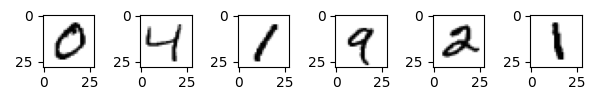
\includegraphics{./pictures/mnist_example.png}}
	\end{center}
	\caption{MNIST dataset example}

	\label{fig:mnist_example}
\end{figure}
To give an impression of the current level of digits recognition algorithms basing on MNIST dataset, several machine learning methods are juxtaposed on the \tablename{}~\ref{tab:mnist_comparison}.
\begin{table}[h!]
\centering
\begin{tabular}{    |l|c|c|c|  }
\hline
  Type & Classifier & Error rate (\%)  \\
 \hline
  Linear classifier & Pairwise linear classifier & \num{7.6} \cite{b:Lecun} \\
 \hline
  K-Nearest Neighbors & K-NN with non-linear deformation (P2DHMDM) & \num{0.52} \cite{b:Keysers} \\
 \hline
   Deep neural network (DNN) & 2-layer 784-800-10 & \num{1.6} \cite{b:Simard} \\
 \hline
   Deep neural network (DNN) & 6-layer 784-2500-2000-1500-1000-500-10 & \num{0.35} \cite{b:Cire_an_2010} \\
 \hline
\end{tabular}
 \caption{Several deep learning algorithms comparison in the digits recognition basing on MNIST database}
\label{tab:mnist_comparison}
\end{table}
It is very easy to take an advantage of this database, whilst working with for example Tensorflow, because the dataset can be downloaded directly using the library API. In this paper MNIST dataset will be exploited only for the training purposes.

\paragraph{How it works}
To goal is to recognise individual handwritten digits (outside the MNIST database) in real time by the camera. The images are captured in Python, resized to the 28x28 size and sent to the embedded system through UART, where deep feed forward neural network is implemented. Detected digit is displayed on the 7 segment display. System provides two ways of preprocessing the images. Adaptive Gaussian thresholding with the help of Open CV's API and Otsu thresholding implemented from the basis both in pure Python and C (in embedded system). Desired preprocessing might be chosen in the main script of communication application (main.py):
\begin{minted}[frame=single, linenos]{python}
class Preprocessing():
    ADAPTIVE_THRESHOLD = 1
    OTSU = 2
    OTSU_ORIGINAL_IMAGE_NO_SERIAL = 3 # no data transfer to the uC -- just 
                                      # for the visualisation. OTSU
                                      # on not resized image, high quality
    OTSU_EMBEDDED = 4
    
###################################################
# configuration part:
###################################################
SERIAL = False
PREPROCESSING = Preprocessing.OTSU_ORIGINAL_IMAGE_NO_SERIAL
\end{minted}
Two variables are to be adapted by the user. If the SERIAL flag is true, data are being sent to the microcontroller, otherwise all process of recognition is done on the PC. User chooses the preprocessing algorithm with the PREPROCESSING variable.

Results evaluation and the whole process of recognition is thoroughly discussed in the following parts of the paper. 

\paragraph{Project structure}
Figure \ref{fig:project structure} presents project structure. It is divided into two main sub projects -- neural\_network with Python and C feed forward implementation in two version: one and two hidden layers, and video, which is an communication project -- main.py contains aforementioned SERIAL and PREPROCESSING configuration, so it directly sends an image content to the microcontroller. 1\_hidden and 2\_hidden contains the same content, but with different amount of neural network hidden layers. 
\begin{figure}[H]
	\begin{center}
		\scalebox{.7}{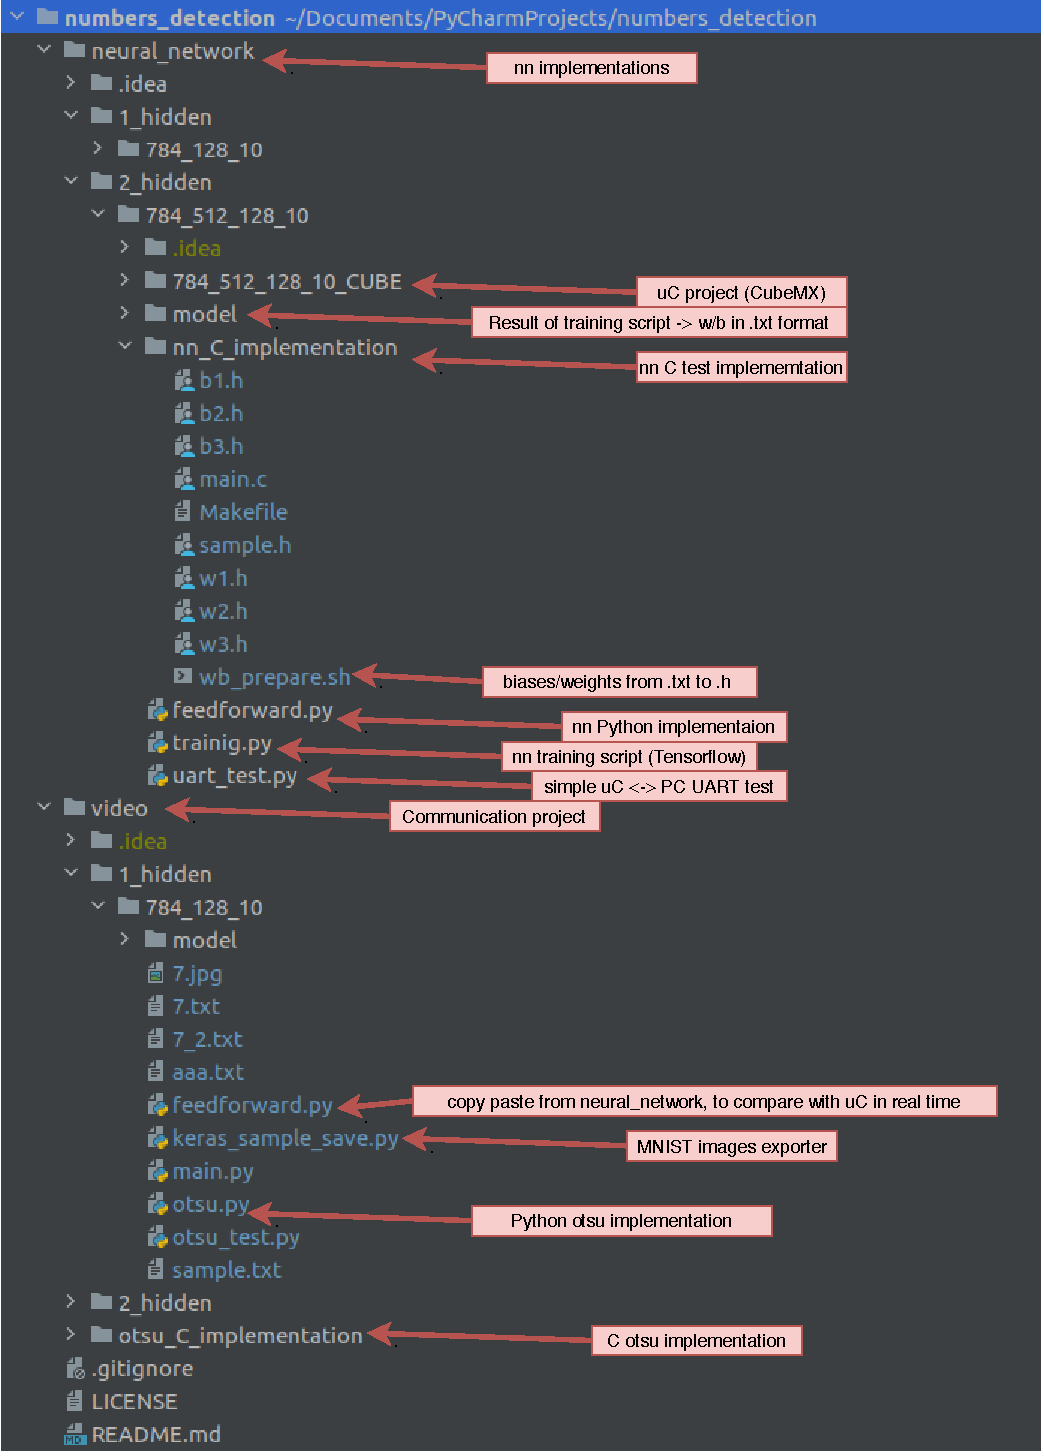
\includegraphics{./pictures/structure.pdf}}
	\end{center}
	\caption{Project structure}

	\label{fig:project structure}
\end{figure}

\begingroup
\renewcommand{\cleardoublepage}{}
\renewcommand{\clearpage}{}
\chapter{Preprocessing}
\endgroup
Training images are provided in the 28x28 array already preprocessed in the MNIST database, however images provided in the real time even though conceptually the same are significantly different. Two first pictures from the left of the \figurename{} \ref{fig:7_images} present digit 7. First one comes from the MNIST database, second one is a raw picture taken by the camera. The difference is in the background of the digit, which is not purely white, what introduces huge distortion in the process of recognition. Background of the original MNIST image in gray scale is zero, background of the raw image is bigger than zero, maybe not high, but still, it makes the neural network which was trained on the MNIST dataset incapable of detecting the digits correctly. Therefore thresholding is necessary.
\begin{figure}[H]
	\begin{center}
		\scalebox{.09}{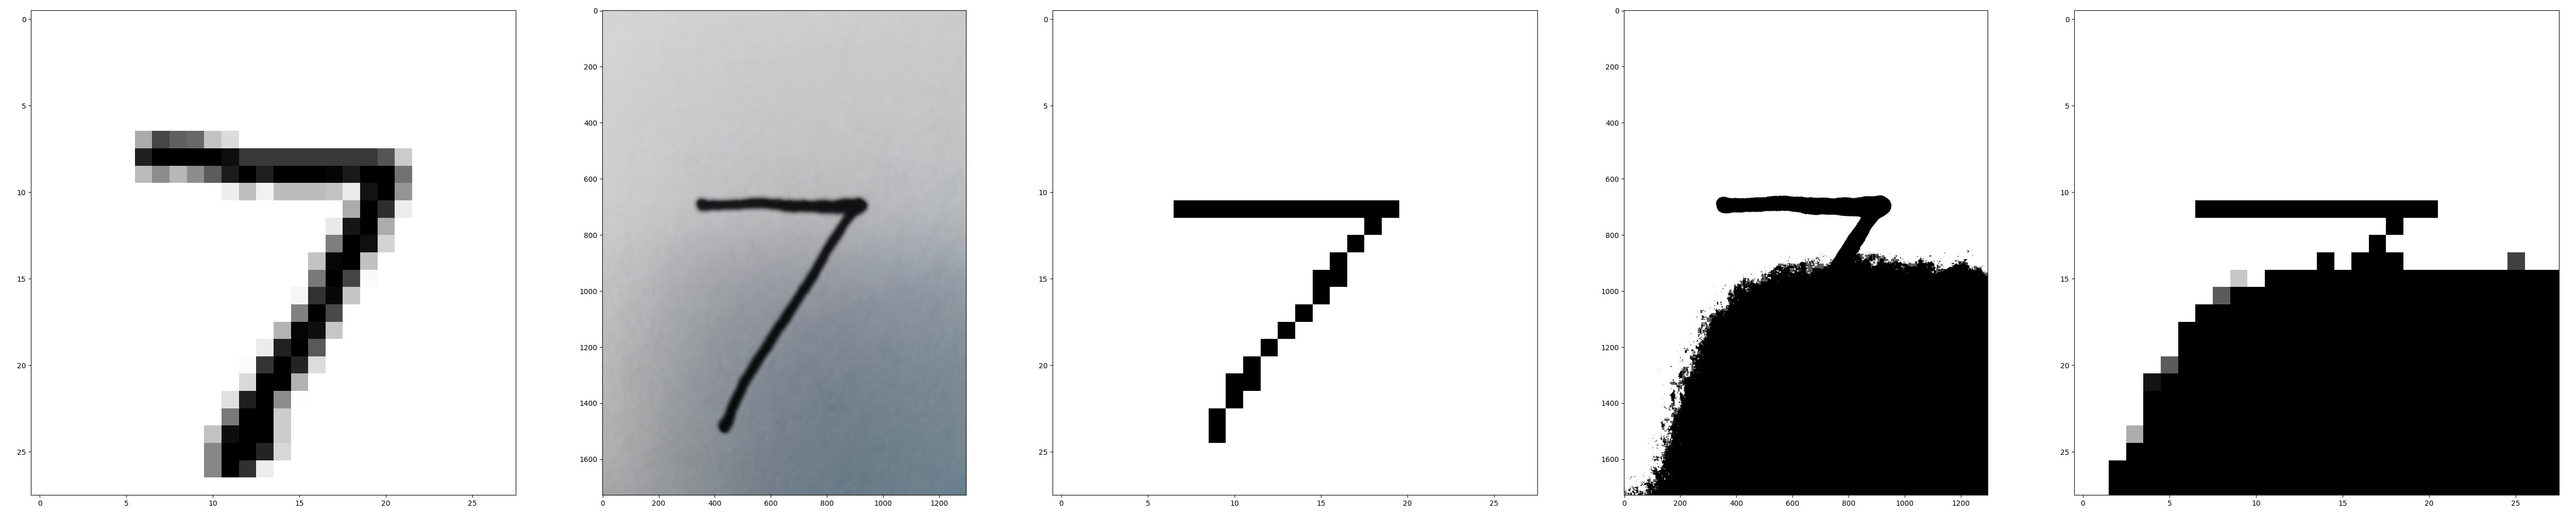
\includegraphics[origin=c]{./pictures/7_images.png}}
	\end{center}
	\caption{Set of preprocessed images. From the left: MNIST example, taken by the camera (raw), adaptive thresholding, Otsu on the original image, Otsu on the previously resized.}
	\label{fig:7_images}
\end{figure}
Image in the centre shows the outcome of adaptive thresholding. This algorithm helps when the lighting conditions are not always the same, which is exactly the case here. The idea is to mute the background and express the digit. Algorithm calculates the threshold for every pixel based on a small region around it. More narrowly it is a gaussian-weighted sum of the pixel's neighbourhood. Pixel with higher value than the threshold is cast to 255 (black), with lower to 0 (white). Open CV provides an API to take an advantage of this thresholding:
\begin{minted}[frame=single, linenos]{python}
arr   = np.asarray(cv2.imread('7.jpg', cv2.IMREAD_GRAYSCALE))
arr2  = cv2.resize(arr, (28, 28))
trunc = cv2.adaptiveThreshold(arr2, 255, cv2.ADAPTIVE_THRESH_GAUSSIAN_C, 
    cv2.THRESH_BINARY_INV, 11, 9)
\end{minted}

\begingroup
\renewcommand{\cleardoublepage}{}
\renewcommand{\clearpage}{}
\section{Otsu}
\endgroup
Otsu method is named after its author Nobuyuki Otsu. Calculated threshold separates the pixels into two classes foreground and background \cite{b:otsu}. The method bases on minimising the between class variance or equally by maximising within class variance, but the first one is significantly faster. \figurename{} \ref{fig:otsu_example} shows the result of Otsu thresholding for the image captured by laptop build-in camera.
\begin{figure}[H]
	\begin{center}
		\scalebox{.5}{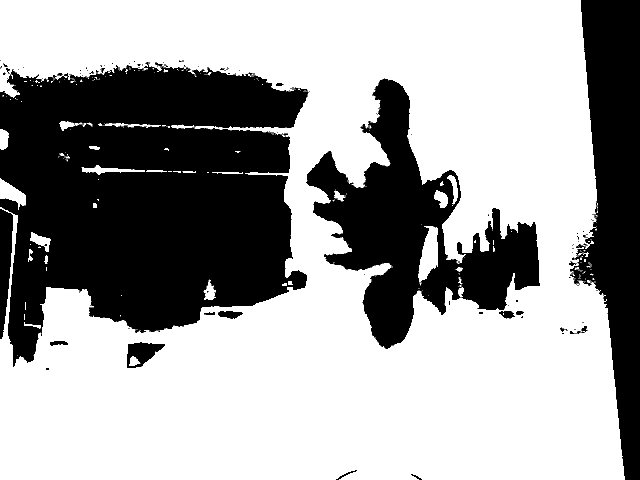
\includegraphics[origin=c]{./pictures/otsu_full_quality.png}}
	\end{center}
	\caption{Image captured by build-in laptop camera processed by Otsu}
	\label{fig:otsu_example}
\end{figure}
\subsection{Algorithm}
The outcome of the method comes down to the division of the whole set of pixels into two classes, foreground and background. Otsu proposed to separate the pixel clusters by maximising the withing class variances, what means maximising the clusters separation. The variance is calculated on the distribution of the pixel intensities, so the histogram of the image, what leads to the probability distribution. This is given by the formula \ref{eq:otsu_1}, where $\sigma_W$ represents within class variance, $\sigma_{b}^{2}$ and $\sigma_{f}^{2}$ variances of the background and foreground classes, $W_b$ and $W_f$ are the probabilities that the classes are separated by the threshold T.
\begin{equation} \label{eq:otsu_1}
\sigma_{W}^{2}(T) = W_b(T)\sigma_{b}^{2}(T) + W_f(T)\sigma_{f}^{2}(T)
\end{equation}
Between class variance is given by the relation \ref{eq:otsu_2}
\begin{equation} \label{eq:otsu_2}
    \sigma_{B}^{2}(T) = \sigma^{2} - \sigma_{W}^{2}(T)
\end{equation}
What finally results (after the calculations) in the relation \ref{eq:otsu_3}, where $\mu_b$ and $\mu_f$ are the weighted means of the particular cluster.
\begin{equation} \label{eq:otsu_3}
    \sigma_{B}^{2}(T) = W_b(T)W_f(T)(\mu_{b}(T) - \mu_{f}(T))^2
\end{equation}
The following listing shows the algorithm implementation in C:
\begin{minted}[frame=single, linenos]{C}
void otsu(int image[], int size) {
    int histogram[BINS_NUMBER] = {0};
    calculate_histogram(histogram, image, size);
    
    float sum = 0;
    for(int i = 0; i < BINS_NUMBER; i++) sum += i*histogram[i];
    
    float sumB = 0, wB = 0, wF = 0, varMax = 0, 
    int threshold = 0;
    for(int t = 0; t < size; t++) {
        wB += histogram[t];
        if(wB == 0) continue;
        wF = size - wB;
        if(wF == 0) break;
        
        sumB += (float)t*histogram[t];
        float mB = sumB / wB;
        float mF = (sum-sumB) / wF;
        float varBetween = wB * wF * (mB-mF)*(mB-mF);
        
        if(varBetween > varMax) {
            varMax = varBetween;
            threshold = t;
        }
    }
    printf("threshold = %d\n", threshold);
    for(int i = 0; i < size; i++) image[i] = image[i] > threshold ? 0 : 255;
}
\end{minted}
Where the histogram is calculated in the following way:
\begin{minted}[frame=single, linenos]{C}
void calculate_histogram(int histogram[], int image[], int size) {
	for(int i = 0; i < size; i++) {
		histogram[image[i]]++;
	}
}
\end{minted}
Two last images from the picture \ref{fig:7_images} present consecutively the result of original image Otsu thresholding and the same image, but previously resized to 28x28 pixels. Adaptive threshold for this image gives better results, however it is not always the case.
\begingroup
\renewcommand{\cleardoublepage}{}
\renewcommand{\clearpage}{}
\chapter{Neural network}
\endgroup
Deep feed forward was chosen as a neural network. Feed forward pass was implemented in pure Python without high level libraries like NumPy or Tensorflow, then reimplemented in C in order to be placed in the microcontroller. However the process of training was outsourced to the Tensorflow in version 2. Weights and biases from the trained multilayer perceptron then are saved in the C header files. 

\section{Feedforward neural network}
Feedforward neural network is a multilayer perceptron with several hidden layers extensively used in machine learning along with deep convolutional neural networks and recurrent neural networks. The forward pass, so the process of thinking is relatively simple and performance effective. \figurename{} \ref{fig:feedforward} shows deep feedforward neural network with multiple inputs and outputs. In the feed forward pass all inputs are multiplied by weights in the connection with the first hidden node what results in the net input $z_1[0]=i[0]w_1[0][0]+i[1]w_1[1][0]+\dots+i[k]w_1[k][0] + b_1[0]$. Subsequently the net input $z$ is applied to the activation function. The process is performed for every node in every hidden and output layer, where output from the particular node is an input of the next node. It is worth noting that the number of nodes in the hidden layers not necessarily has to be equal. Formal process of the feed forward pass for particular the node is written in \ref{eq:feedforward}, where $f_k$ represents activation function for the layer $k$ which is either ReLU for hidden layers or sigmoid for the output one. Rectified linear unit (ReLU) has an advantage over sigmoid function used in the output layer, because it does not have vanishing gradient, which prevents neural network from efficient learning. In fact ReLU has the constant gradient. Sigmoid activation function is given by \ref{eq:sigmoid}, whereas ReLU by \ref{eq:ReLU}.

\begin{equation} \label{eq:feedforward}
\begin{aligned}
    z_k[0]&=n_{k-1}[0]w_k[0][0]+n_{k-1}[1]w_k[1][0]+\dots+n_{k-1}[m]w_k[m][0] + b_k[0] \\
    n_k[0]&=f_k(z_k[0]) \\
\end{aligned}
\end{equation}

\begin{equation} \label{eq:sigmoid}
f(z)=\frac{1}{1-e^{-z}}
\end{equation}

\begin{equation} \label{eq:ReLU}
f(z)=max(0, z)
\end{equation}

\begin{figure}[H]
	\begin{center}
		\scalebox{.6}{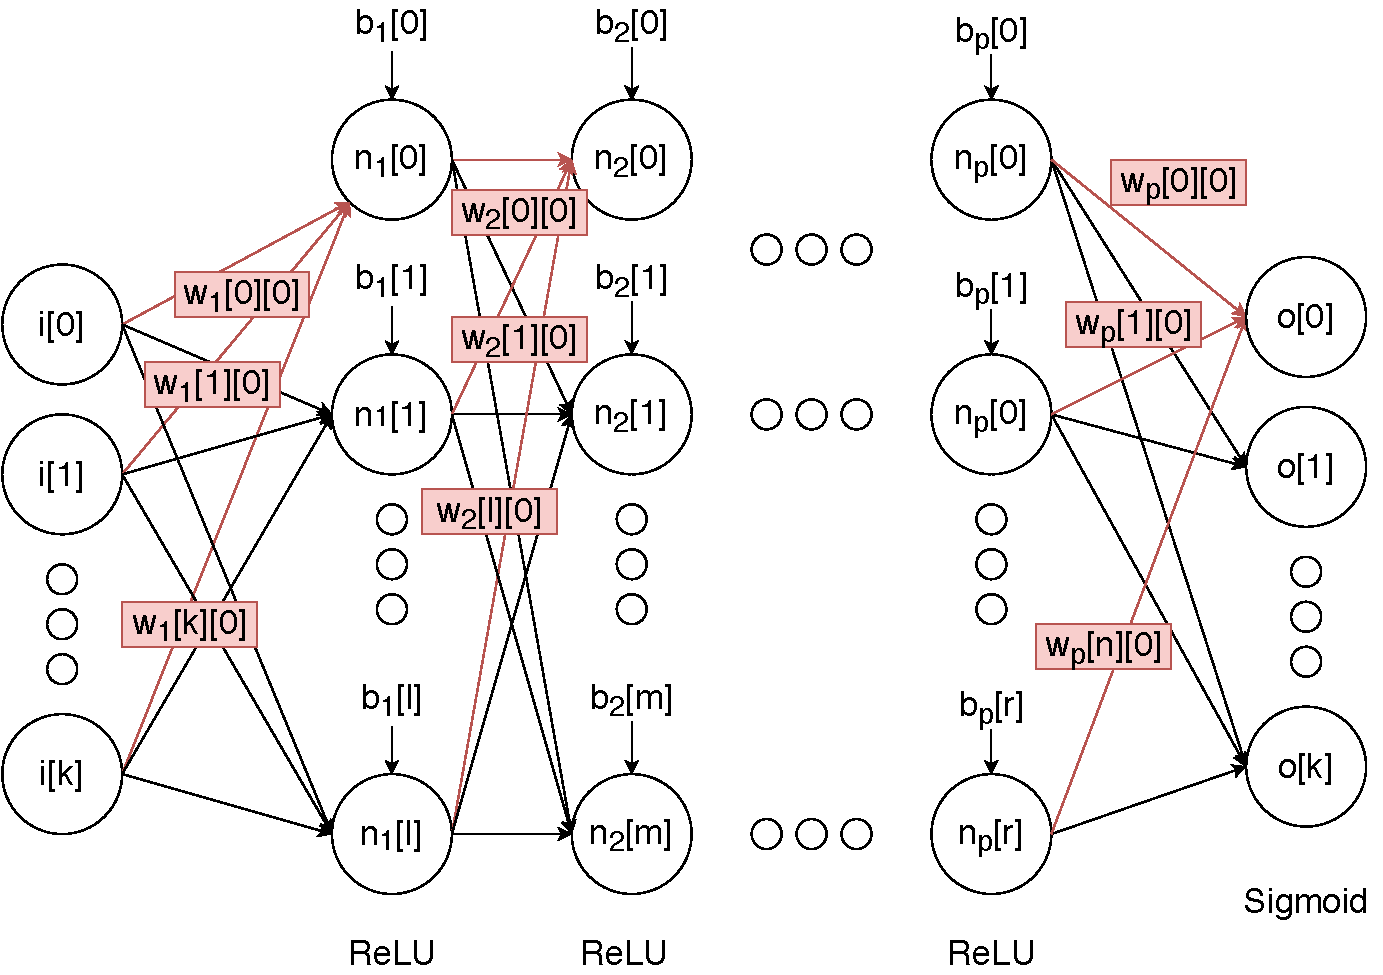
\includegraphics{./pictures/feedforward.pdf}}
	\end{center}
	\caption{Feedforward neural network with multiple inputs and outputs. On the bottom of every layer, activation function was presented.}

	\label{fig:feedforward}
\end{figure}
Python implementation of the feedforward pass is presented on the following listing. This function is invoked for every hidden and output layer. Then the result of particular layer is passed to the consecutive one.
\begin{minted}[frame=single, linenos]{python}
def feedForward(self, inputs, weights_matrix, biases, activationFunction):
    input_length = len(weights_matrix)
    output_length = len(weights_matrix[0])
    x = inputs
    y = []
    z = []  # without activation
    
    for o in range(0, output_length):  # calculate each output in order
        y.append(0)
        z.append(0)
        for i in range(0, input_length): 
            y[o] += weights_matrix[i][o] * x[i]
    
        z[o] = y[o] + biases[o]
    
    for o in range(0, output_length):
        y[o] = activationFunction(z[o])
    
    return y, z
\end{minted}
And the process of thinking, so the way of feedForward invocation for the consecutive layers. In the example 1 hidden layer.
\begin{minted}[frame=single, linenos]{python}
def think(self, x):
    (self.l1_output, self.l1_z) = self.feedForward(x, self.w1, self.b1, 
        self.ReLU)
    (self.output, self.output_z) = self.feedForward(self.l1_output, self.w2, 
        self.b2, self.sigmoid)
    return self.output
\end{minted}
Following two listings show the implementation in C which are directly used by the microcontroller. Moving from Python to C is not trivial in this case, because two dimensional weights matrix is expressed in one dimension. Otherwise it would not be possible to pass different sizes of this matrix. Particular weight is obtained in the line 9. Activation function is passed as a function pointer. 
\begin{minted}[frame=single, linenos]{C}
void feedforward(const double x[], double z[], const double weights_matrix[], 
    int ROW, int COL, const double biases[], double y[],
    double (*activationFunction)(double)) {
	int o, i;
	double cur_w;

	for(o = 0; o < COL; o++) {
		for(i = 0; i < ROW; i++) {
			cur_w = *(weights_matrix + i*COL + o);
			y[o] += cur_w * x[i];
		}

		z[o] = y[o] + biases[o];
	}

	for(o = 0; o < COL; o++) {
		y[o] = (*activationFunction)(z[o]);
	}
}
\end{minted}
And the process of thinking:
\begin{minted}[frame=single, linenos]{C}
void think(const double x[], double y[], double z[]) {
	double l1_output[128] = {0}, z1[128] = {0};
	feedforward(x        , z1, w1[0], 784, 128, b1, l1_output, &ReLU);
	feedforward(l1_output, z,  w2[0], 128, 10,  b2, y, &sigmoid);
}
\end{minted}
\section{Training process}
Training was performed using Tensorflow library in the version 2.2 however implementation in pure Python is also provided (check Appendix \ref{ch:back}). Time of the training varies between several seconds to roughly a few minutes, depending on the amount of epochs, nodes in the particular layer and the layers itself. Neural network is fully connected. As a lost function sparse categorical cross entropy was used, because the classes are mutually exclusive. It is given by the formula \ref{eq:bce}, where $y_a$ and $y_d$ are the actual outputs of the neural network respectively and $L$ is the loss function.
\begin{equation} \label{eq:bce}
L(y_a,y_d)=-\frac{1}{N}\sum_{i=1}^{N}[y_{a_i}log(y_{d_i})+(1-y_{a_i})log(1-y_{d_i})]
\end{equation}
The training process starts with the model definition, goes through the training itself and finally finishes on the model saving as well as the weights and biases in the proper format. The following listing shows the training implementation for 1 hidden layer with 128 nodes, input with $28\cdot28=784$ nodes and 10 output neurons.
\begin{minted}[frame=single, linenos]{python}
def createModel(self):
    self.model = keras.Sequential([ # layers in sequence
                 keras.layers.Flatten(input_shape=(28, 28)),
                 keras.layers.Dense(128, activation="relu"),  # fully connected
                 keras.layers.Dense(10, activation="sigmoid")
            ])
    self.model.compile(optimizer="adam", 
    loss="sparse_categorical_crossentropy", metrics=["accuracy"])

def trainModel(self, epochs_num, save=True):
    self.model.fit(self.train_data, self.train_labels, epochs=epochs_num)
    test_loss, test_acc = self.model.evaluate(self.test_data, self.test_labels)
\end{minted}
Training takes an advantage of MNIST database as it was already aforementioned. When loaded, images are scaled to the range of 0-1.
\begin{minted}[frame=single, linenos]{python}
(self.train_data, self.train_labels), (self.test_data, self.test_labels) = 
    keras.datasets.mnist.load_data()
self.train_data = self.train_data / 255.0
self.test_data = self.test_data / 255.0
\end{minted}
Weights and biases are saved in the proper format, more narrowly they are exported to the .txt file along with the whole model and then transformed to the header files with the help of regexp and specially designed bash script.


\begingroup
\renewcommand{\cleardoublepage}{}
\renewcommand{\clearpage}{}
\chapter{PC side}
\endgroup
In this project camera is directly connected to the PC, but may be external one. The images are captured in real time, resized and depending on the need directly sent to the microcontroller or previously preprocessed. All of that is implemented in Python 3 with the help of OpenCV and serial package. The following listing shows the serial configuration.
\begin{minted}[frame=single, linenos]{python}
ser = serial.Serial(
    port='/dev/ttyACM0',
    baudrate=115200,
    parity=serial.PARITY_NONE,
    stopbits=serial.STOPBITS_ONE,
    bytesize=serial.EIGHTBITS
)
\end{minted}
When the picture is ready to be sent it is flattened, that is changed to one dimensional array. Then every pixel is packed in 3 bytes format and sent. Synchronisation with the microcontroller is sygnalised by 2 special values: "aaa" stands for the beginning of the transfer and "bbb" for the end. Right after the beginning characters 3 bytes distinguishing the process of preprocessing are sent -- "OOO" in case of Otsu implemented on embedded system, "AAA" otherwise (outside microcontroller) for example adaptive thresholding. 
\begin{minted}[frame=single, linenos]{python}
def send(ser, data, type):
    ser.write("aaa".encode())
    if type == Preprocessing.OTSU_EMBEDDED:
        ser.write("OOO".encode())
    else:
        ser.write("AAA".encode())

    for i in data.flatten():
        to_send = '{:3d}'.format(i)
        ser.write(to_send.encode())
    ser.write("bbb".encode())
\end{minted}
It is worth to mention, that the bottleneck of the system is exactly the communication part. Even with the maximum baud rate accessible for UART, sending roughly $28\cdot28\cdot3 + 6$ bytes takes significant amount of time (around \num{1.5} second) which stops systems fluency. Time of neural network computation comparing to this is negligible. 

\begingroup
\renewcommand{\cleardoublepage}{}
\renewcommand{\clearpage}{}
\chapter{Microcontroller}
\endgroup
Neural network and the whole process of recognition is implemented on the microcontroller STM32H743ZIT6U. Embedded system is placed on the Nucleo board, which is directly connected to the computer through USB. The board was chosen mostly because of high volume of memory. It has 2 Mbytes of Flash memory, where weights and biases resides in the constant arrays and 1 Mbyte SRAM where is the rest of the program, image array for instance. Moreover the core of this device is highly efficient ARM Cortex-M7 at 480MHz, which is desired from the neural network calculations point of view. Figure \ref{fig:STM32H743ZIT6U} presents the Nucleo board with 7 segment display showing number 5.
\begin{figure}[H]
	\begin{center}
		\scalebox{.18}{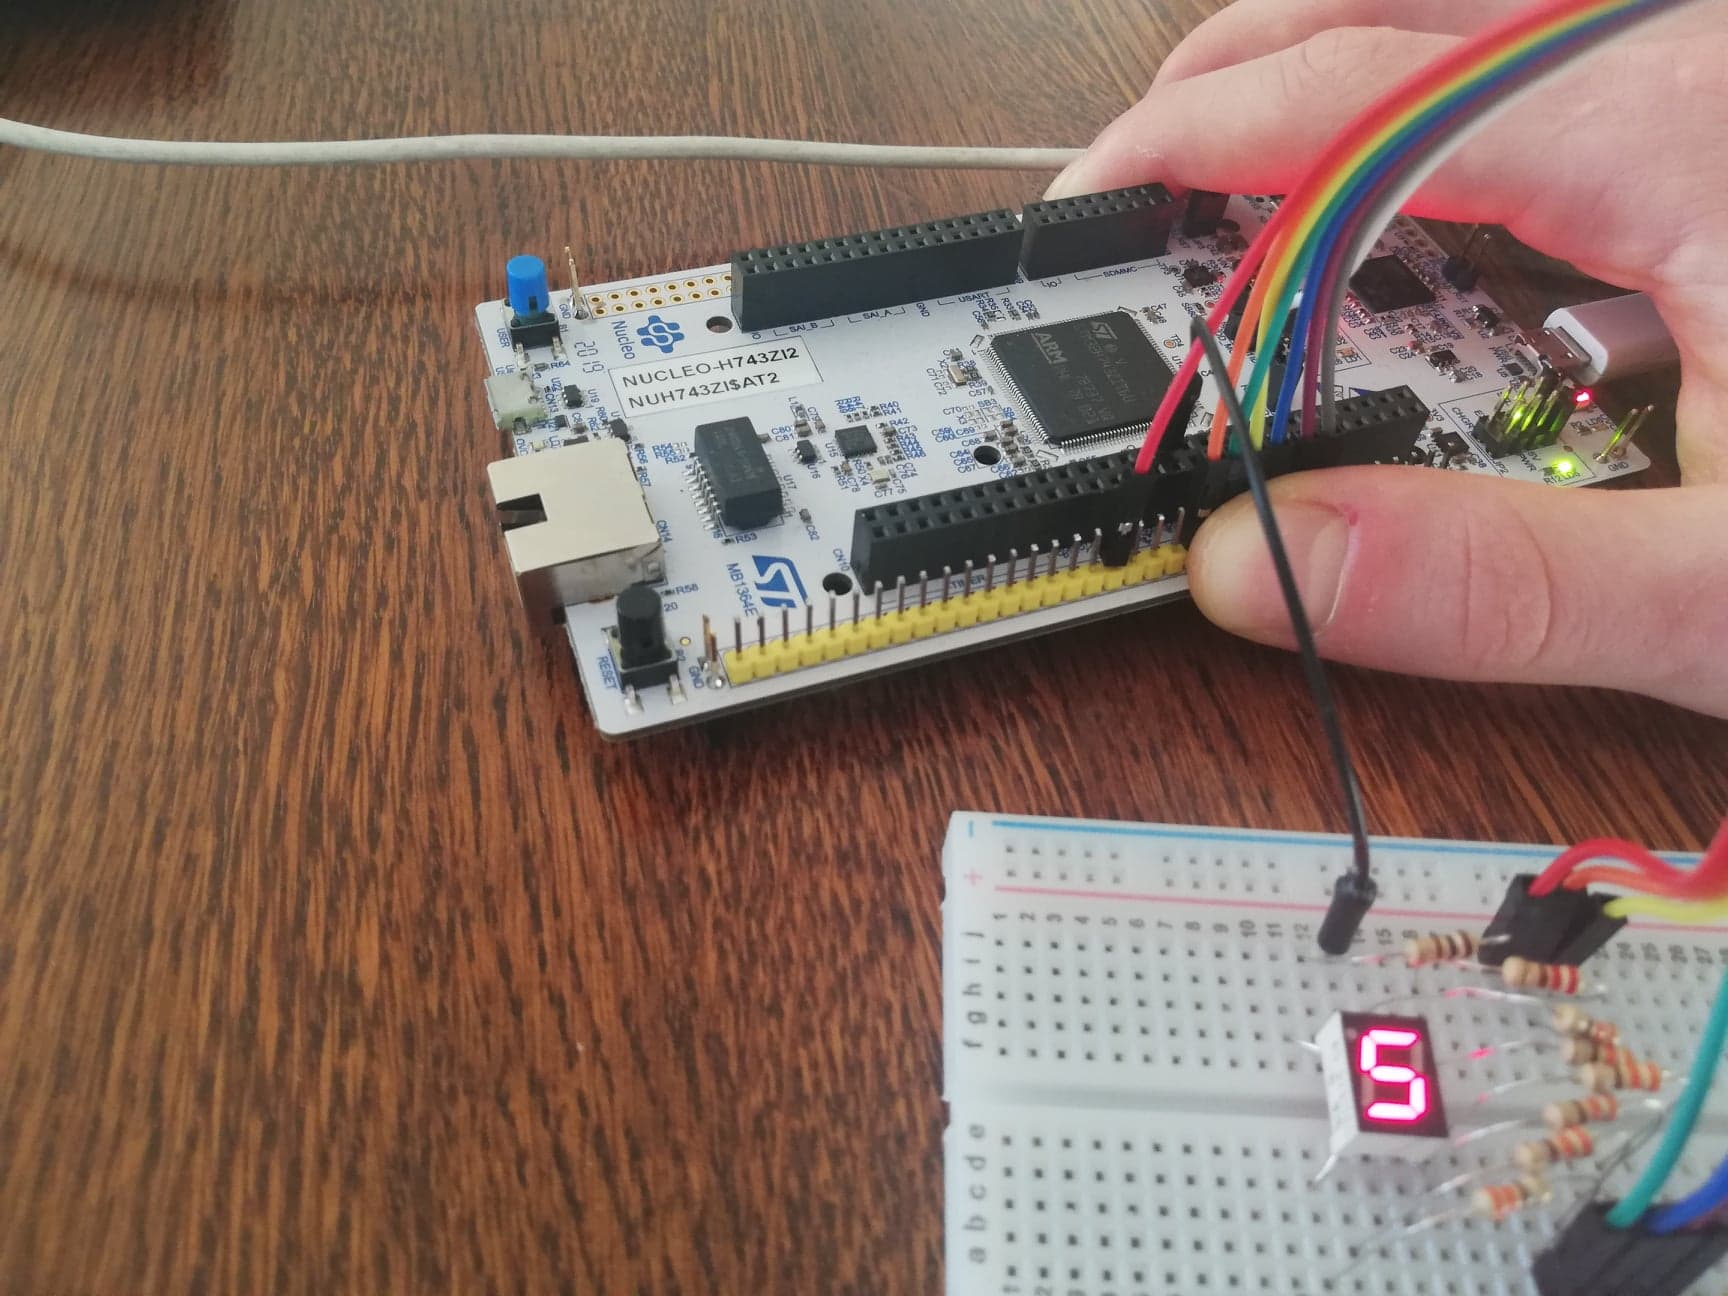
\includegraphics[origin=c]{./pictures/uC.jpg}}
	\end{center}
	\caption{STM32H743ZIT6U with 7 segment display, which shows number 5 as a result of the image recognition}
	\label{fig:STM32H743ZIT6U}
\end{figure}

\begin{figure}[H]
	\begin{center}
		\scalebox{.4}{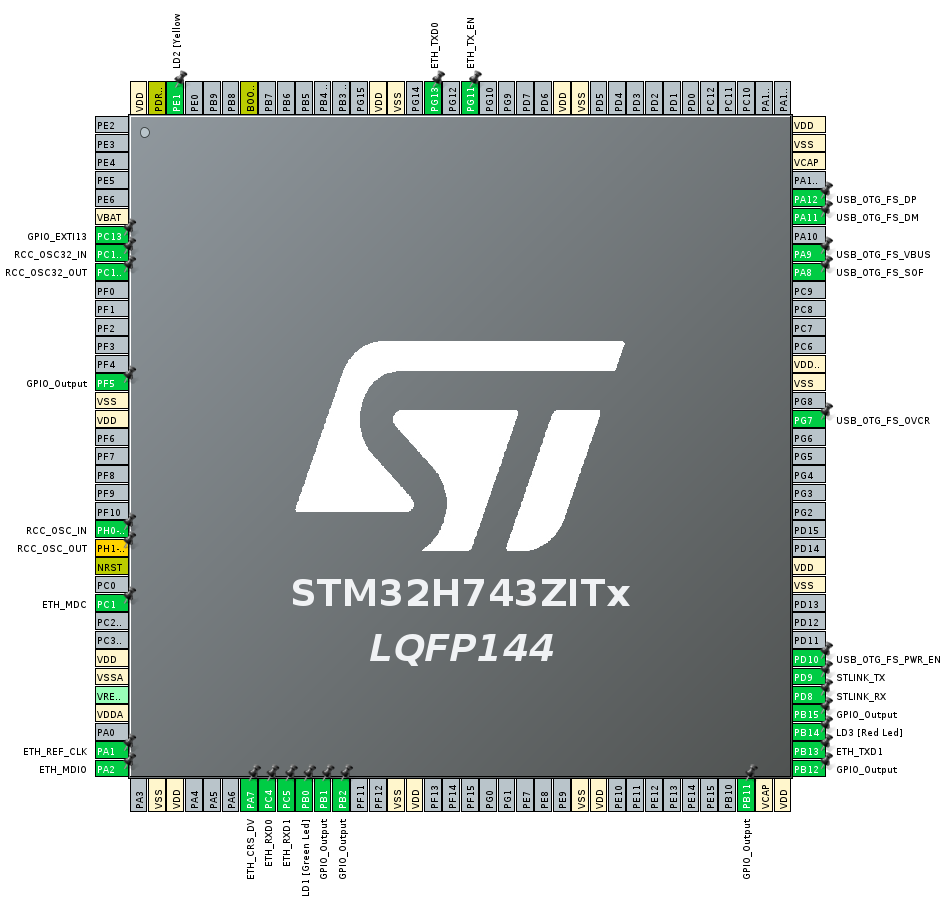
\includegraphics[origin=c]{./pictures/cube_config.png}}
	\end{center}
	\caption{Peripherals STM32CubeMX configuration}
	\label{fig:cube}
\end{figure}
The explanation of the whole process of peripherals configuration is omitted to focus mainly on the program logic. Nevertheless STM32CubeMX peripherals assignment is presented on the \figurename{} \ref{fig:cube}.
Microcontroller's main loop is responsible mainly for the neural network feed forward pass. Nevertheless apart from that there are a few operation worth to explain. First of all "done" flag indicates the end of the image transfer through UART. This flag is set in the interrupt callback, hence volatile. Subsequently Otsu preprocessing is done depending if it is requested via UART message ("OOO" bytes), this flag is also set in the interrupt callback handler. When it is done, image is rescaled and the process of recognition is performed. The result is displayed on the 7 segment display and finally the readiness of transfer is signalised by setting done flag to false. 
\begin{minted}[frame=single, linenos]{C}
#define IMAGE_SIZE 784
uint8_t Received[3];
double image[IMAGE_SIZE];
volatile bool done = false;
volatile bool is_otsu = false;
////
while (1) {
    if(done) {
        if(is_otsu) {
            otsu(image, IMAGE_SIZE);
        }
        
        for(int i = 0; i < IMAGE_SIZE; i++) {
            image[i] = image[i] / 255.0;
        }
    
        think(image, y, z);
        display_digit(max_idx(y));
        done = false;
    }
}
\end{minted}
Interrupt handler for the UART receive event is presented on the following listing. The logic is similar to the process of sending the messages in the communication program, discussed previously. Start and finish flag, "a" (first letter of "aaa"), "b" consecutively. Type of the preprocessing, and the image content itself. Passing around 2000 bytes through UART is a bottleneck of the system as it was already stated. Interrupts introduce the notion of overlapping of the two images transmission -- during the detection of the first one, second image may be being transmitted. However the question is why not to exploit the DMA? Unfortunately there are several issues with DMA in this type of STM32 \footnote{\url{https://community.st.com/s/article/FAQ-DMA-is-not-working-on-STM32H7-devices}}, so the notion of using it was abandoned.
\begin{minted}[frame=single, linenos]{C}
int counter = 0;

void HAL_UART_RxCpltCallback(UART_HandleTypeDef *huart) {
	if(Received[0] == 'a') {
		counter = 0;
	} else
	if(Received[0] == 'b') {
		done = true;
	} else
	if(Received[0] == 'O') {
		is_otsu = true;
	} else
	if(Received[0] == 'A') {
		is_otsu = false;
	} else {
		int value = atoi((const char*)Received);
		image[counter++] = (double)value;
	}

	HAL_UART_Receive_IT(&huart3, Received, 3);
}
\end{minted}

\begingroup
\renewcommand{\cleardoublepage}{}
\renewcommand{\clearpage}{}
\chapter{Experiments and results}
\endgroup
Feed forward with one hidden and 2 hidden layers was tested. More layers could not fit in the microcontroller's flash memory. First of all accuracy of the training process on the MNIST database is presented on the \tablename{}~\ref{tab:mnist_comparison2}.
\begin{table}[h!]
\centering
\begin{tabular}{    |l|c|c|c|c|  }
\hline
  Type & Classifier & Accuracy (\%)  & Epochs number & Loss \\
 \hline
   Feed forward & 1-layer 784-800-10 & \num{0.9721} & 5 & \num{0.0864} \\
 \hline
   Deep feed forward & 2-layer 784-512-128-10 & \num{0.9793} & 5 & \num{0.0727} \\
 \hline
\end{tabular}
 \caption{1 hidden and 2 hidden layers training results}
\label{tab:mnist_comparison2}
\end{table}
Admittedly the training quality rates, namely accuracy and loss (sparse categorical cross entropy) are similar. However one has to remember, that the training was performed on the MNIST database, but the real testing is in the real time, with hand written, subsequently preprocessed images. From the quality point of view, so how two neural networks behave in such conditions, they are capable of detecting the digits correctly. Deep feed forward neural network from the user experience behaves better than 1 hidden layer neural network, in the same time characterising by the similar performance. It is difficult to evaluate the efficiency quantitatively without huge set of images. Same applies to the preprocessing algorithms. Both of them are able to preprocessed the images satisfactory nonetheless. However as it might have been observed on the Figure \ref{fig:7_images}, Otsu is highly vulnerable for lighting differences, hence from time to time some part of the digit may not be exposed correctly (last two images on the Figure \ref{fig:7_images}). As an attachment to this report several test recordings may be found in the projects repository\footnote{\url{https://gitlab-stud.elka.pw.edu.pl/jwieczo1/numbers_detection}}.

\begingroup
\renewcommand{\cleardoublepage}{}
\renewcommand{\clearpage}{}
\chapter{Conclusions}
\endgroup
In this project deep feed forward neural network was implemented on the embedded system for the sake of visual recognition. Nowadays the biggest obstacle for deep learning algorithms is not the performance of the microcontroller, but the memory volume. Even with 2 Mbytes of the flash memory, it was possible to place there only 2 hidden layers. The bottleneck of the system is the image transfer to the STM32, therefore in the future improvement USB protocol is worth considering. Neural networks were trained basing on MNIST dataset instead of specially prepared images. Nevertheless preprocessing approximated the images captured in the real time, so it was not a problem for the detection. It is worth noting, that a digit should be placed in the centre of the camera to be correctly read.

In addition to the neural network two preprocessing algorithms were compared, where Otsu was implemented from the basis and placed onto microcontroller. Adaptive threshold is more resistant to the light differences, so it behaves slightly better. 

\begin{appendices}

\begingroup
\renewcommand{\cleardoublepage}{}
\renewcommand{\clearpage}{}
\chapter{Back propagation} \label{ch:back}
\endgroup
The following appendix shows an implementation of the one hidden layer feed forward back propagation algorithm. Without high level libraries, just pure Python. The difficulties in algorithm implementation grow with the number of layers, because back propagation bases on the gradient calculation, where particular gradient in the layer depends on many factors in the following layers. Thus, for the need of the project back propagation was outsourced to the Tensorflow.
\section{Output layer}
\begin{minted}[frame=single, linenos]{python}
def gradientsOutput(self, inputs, dedo, w, dActivationFunction, acti_arg1):
    """
    @param inputs, The outputs of the last hidden layer
    @param dedo,   Error gradient with respect to the output
    @param w,      An array of weights between output and the 
                   hidden layer. Is constant
    @param dActivationFunction in the case of this layer is 
                   dSigmoid 
    @param acti_arg1 Argument for dActivationFunction. In this case
                   an output of the last layer
    """
    outputs_length = len(w[0])
    inputs_length = len(w)

    dedw = [[0 for o in range(outputs_length)] for i in range(inputs_length)]
    dedb = [0 for o in range(outputs_length)]
    for o in range(0, outputs_length): 
        for i in range(0, inputs_length):
            dedw[i][o] = dedo[o] * dActivationFunction(acti_arg1[o])*inputs[i]
        
        dedb[o] = dedo[o] * dActivationFunction(acti_arg1[o]) * 1
    return dedw, dedb
\end{minted}
\section{Hidden layer}
\begin{minted}[frame=single, linenos]{python}
def gradients(self, inputs, dedo, w, w2, dActivationFunction, acti_arg1, 
    dActivationFunction_2, acti_arg1_2):
    """
    @param inputs, The input of the nn
    @param dedo,   Error gradient with respect to the output
    @param w,      An array of weights between input and the 
                   hidden layer. Is constant
    @param w2,     An array of weights between hidden layer
                   and the output. Gradient of w depends on them.
                   Is constant
    @param dActivationFunction activation for the hidden layer
    @param acti_arg1 Argument for dActivationFunction. If ReLU then
           should be net inputs z.
    @param dActivationFunction2 activation for the output layer
    @param acti_arg2 Argument for dActivationFunction2. 
    """
    outputs_length = len(w[0]) # of w!
    inputs_length = len(w)

    dedw = [[0 for o in range(outputs_length)] for i in range(inputs_length)]
    dedb = [0 for o in range(outputs_length)]
    
    dedohw = [[0 for o in range(outputs_length)] for i in range(inputs_length)]
    dedohb = [0 for o in range(outputs_length)]
    
    outputs_length2 = len(w2[0])
    inputs_length2 = len(w2)

    for o2 in range(0, outputs_length2):
        dEdActiv = dedo[o2] * dActivationFunction_2(acti_arg1_2[o2])
        for o in range(0, outputs_length):
            dedoh = dEdActiv * w2[o][o2]
            for i in range(0, inputs_length):
                dedohw[i][o] += dedoh
            
            dedohb[o] += dedoh

    for o in range(0, outputs_length):
        dActiv = dActivationFunction(acti_arg1[o])
        for i in range(0, inputs_length):
            dedw[i][o] = dedohw[i][o] * dActiv * inputs[i]
        
        dedb[o] = dedohb[o] * dActiv * 1

    return dedw, dedb
\end{minted}
\section{Back propagation chain}
\begin{minted}[frame=single, linenos]{python}
def learn(self, x, y_desired):
    y = self.think(x)
    dedo = self.dSqe(y, y_desired)

    (dedw2, dedb2) = self.gradientsOutput(self.l1_output, dedo, self.w2, 
        self.dSigmoid, self.output)
    (dedw1, dedb1) = self.gradients(x, dedo, self.w1, self.w2, 
        self.dReLU, self.l1_z, self.dSigmoid, self.output)
    
    self.update(self.w2, self.b2, dedw2, dedb2)
    self.update(self.w1, self.b1, dedw1, dedb1)
\end{minted}

\section{Update function}
\begin{minted}[frame=single, linenos]{python}
def update(self, w, b, dedw, dedb):
    outputs_length = len(w[0])
    inputs_length = len(w)
    
    for o in range(0, outputs_length):
        for i in range(0, inputs_length):
            w[i][o] += dedw[i][o] * self.lr
        
        b[o] += dedb[o] * self.lr
\end{minted}

\end{appendices}